
\documentclass[12pt]{article}

\usepackage[margin=0.85in,footskip=0.25in]{geometry}

\usepackage{xcolor} 
\definecolor{grey}{rgb}{0.9,0.9,0.9}

\usepackage[scaled]{helvet}
\usepackage[T1]{fontenc}

\usepackage{graphicx, float}
\usepackage{caption}
\usepackage{hyperref}


\begin{document}

\begin{titlepage} 
	\colorbox{grey}{
		\parbox[t]{0.93\textwidth}{ 
			\parbox[t]{0.91\textwidth}{ 
				\raggedleft 
				\fontsize{50pt}{80pt}\selectfont 
				\vspace{0.7cm} 				
				A Primer Into USB Type-C\\
				for Legacy USB2 Applications\\
				and Simple Power Delivery\\
				
				\vspace{0.7cm} 
			}
		}
	}
	
	\vfill 		
	\parbox[t]{0.93\textwidth}{ 
		\raggedleft 
		\large 
		{\Large Hugo Hu}\\[4pt]
		\texttt{v1.0.1 released 11/03/2023}\\
		\texttt{\href{mailto:hugo@hugohu.me}{hugo@hugohu.me}}\\
		\texttt{\href{https://hugohu.me}{hugohu.me}}\\
		
		\hfill\rule{0.2\linewidth}{1pt}
	}
	
\end{titlepage}


\tableofcontents
\newpage
\section{Introduction}
\subsection{"I've been living under a rock since 2014, what's USB-C?"}

USB-C is the most modern USB connector from the last decade. It supersedes all previous USB connector versions. It is backwards-compatible with previous USB-generations and all new ones are designed around it (including USB3 and USB4). \\\\
\noindent
Also, it's reversible! The USB-C connector has a total of 12 pins: two GND, two VBUS, a USB2.0 pair, a SuperSpeed TX pair, a SuperSpeed RX pair, a Configuration Channel (CC) pin and a Sideband Use(SBU) pin. Since the connector is reversible, there are a total of 24 pins on the connector itself (12 on the top, 12 on the bottom). \\\\
\noindent
USB-C allows for extraordinary data and power transfer better than anything in previous generations. USB4 can support 40Gbps (theoretically 80Gbps with USB4 Gen 4) and power delivery up to 100W (Standard Power Range, 20V @ 5A) or 240W (Extended Power Range, 48V @ 5A).  \\\\
\begin{figure}[h]
	\centering
	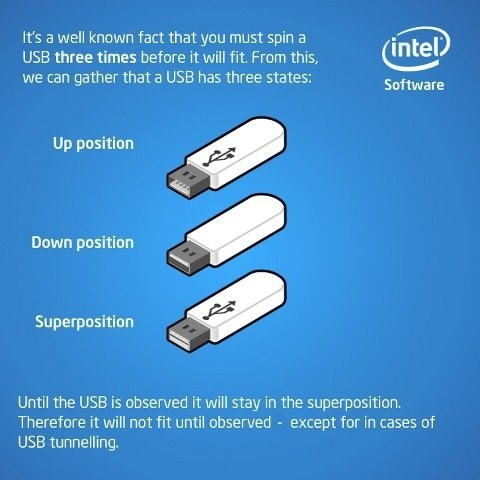
\includegraphics[width=0.6\linewidth]{images/intel.jpg}
	\caption{Rumors say that Intel made this ad themselves.}
	\captionsetup{justification=raggedright,singlelinecheck=false}
	\label{fig:usbSuperposition}
\end{figure}


\subsection{OK... and?}
Since USB-C is backwards compatible with USB2 and even USB1.1, it should be pretty darn simple to just put in a new connector and rework the circuit, right?\\\\
\noindent
Well, no. In 2019, the Raspberry Pi Foundation released the Raspberry Pi 4B- a powerful upgrade over the 3B+, and added USB-C to replace the micro-B power input. \\\\
\noindent
The TL;DR is, they messed up. Instead of connecting separate resistors for the CC pins, they shorted the pins, which didn't allow power input for e-marked cables. Oops. 

\section{Converting USB2 to USB-C}
Here's how a USB2 micro-B receptacle would be wired up (assuming it's a device):

\begin{figure}[h]
	\centering
	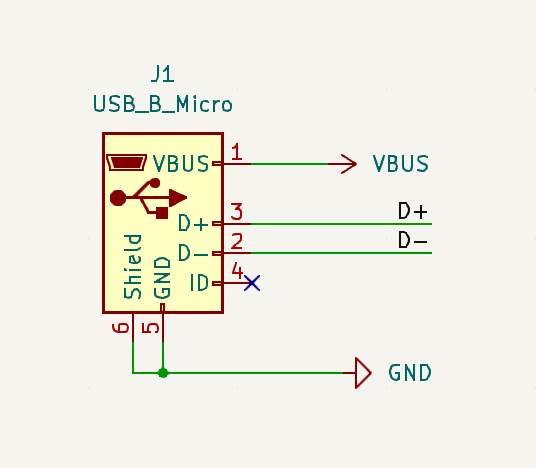
\includegraphics[width=0.43\linewidth]{images/USB-micro-B.png}
	\caption{USB2 micro-B female port wiring.}
	\label{fig:usb2_microB}
\end{figure}

A \textbf{incorrect} wiring to implement the same USB 2 signal through USB-C:

\begin{figure}[h]
	\centering
	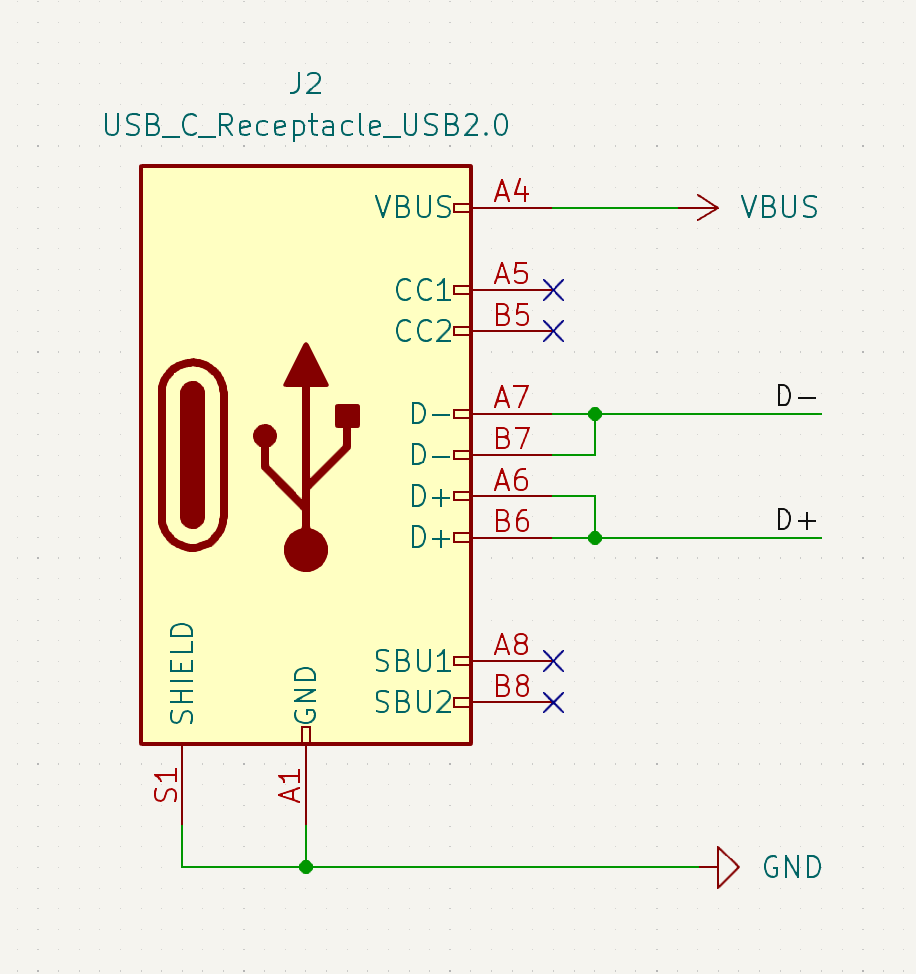
\includegraphics[width=0.43\linewidth]{images/USB-faulty-type-C.png}
	\caption{Faulty USB2 Type-C wiring.}
	\label{fig:usb2_faulty_usbc}
\end{figure} 

\noindent 
This breaks out the D- and D+ pins, the VBUS pin, and GND. This should work!\\\\
\noindent
Unfortunately, it doesn't. This would make your board perfectly OK with legacy non e-marked cables, but would not work with a "smart" e-marked cable. The reason for this is because USB-C requires you to negotiate for power. For legacy applications, your power source doesn't have this ability, so it just defaults to 5V @ 500mA(USB2.0) or 900mA(USB3.0). \\\\
\noindent
With Power Delivery, you can essentially request a certain voltage and current from a PD-compatible source. One example is the \href{https://www.apple.com/shop/product/MHJA3AM/A/20w-usb-c-power-adapter}{\$19 Apple 20W Power Brick} which supports PD, capable of 5V@3A or 9V@2.22A. 

\subsection{Analog Power Negotiation} \label{sec:AnalogPower}
In order to request voltage, digital negotiation on the CC pin is required to negotiate for any voltage option above 5V. This clearly doesn't make sense to implement a chip like the \href{https://www.infineon.com/dgdl/Infineon-EZ-PD_BCR_Datasheet_USB_Type-C_Port_Controller_for_Power_Sinks-DataSheet-v03_00-EN.pdf?fileId=8ac78c8c7d0d8da4017d0ee7ce9d70ad}{CYPD3177-24LQXQ} that adds cost and complexity just to get 5V for a legacy USB2 application. That's stupid.\\\\
\noindent
Fear not. There's a cheap way to negotiate for additional current flow for USB Type-C charging at 1.5A@5V or 3.0A@5V. You might ask, "if I don't need more than 500mA, can't I leave the CC pins unpopulated?" No: CC pulldown resistors are required for a power source to enable VBUS at all. You need a 5.1K$\Omega$ ± 10\% pulldown resistor on each CC pin (no, you cannot short CC1 and CC2) for a total of two resistors added. Not terrible, and pretty cheap. You'll get 5V as expected on VBUS making switching an older connector to USB-C as easy as adding in the connector and two pulldown resistors. Everything else in your circuit can stay the same.

\begin{figure}[h]
	\centering
	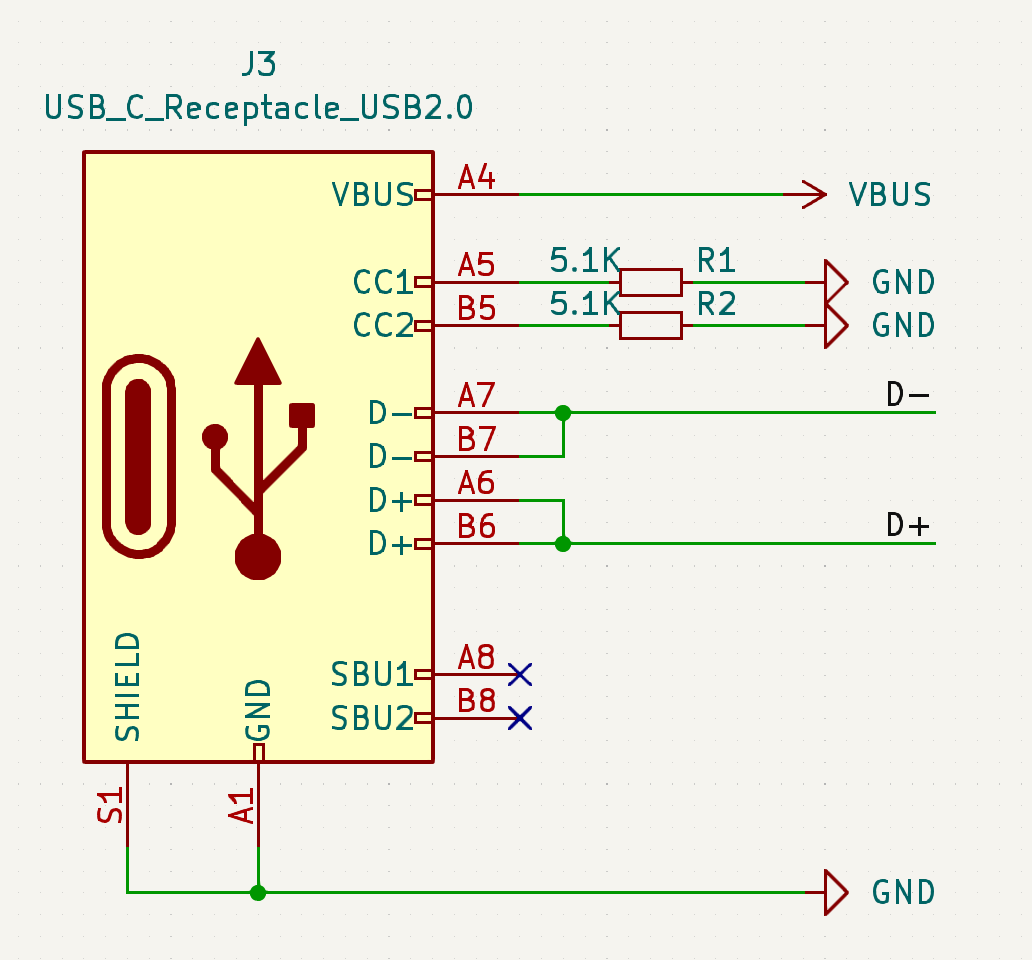
\includegraphics[width=0.55\linewidth]{images/USB-C-Pulldown.png}
	\caption{USB2 Type-C with 5V}
	\label{fig:usb2_5V_usbc}
\end{figure}



\section{Picking a Connector}

There are a variety of connectors you can pick for USB-C: Power-Only, USB2, and USB3. 

\begin{figure}[h]
	\centering
	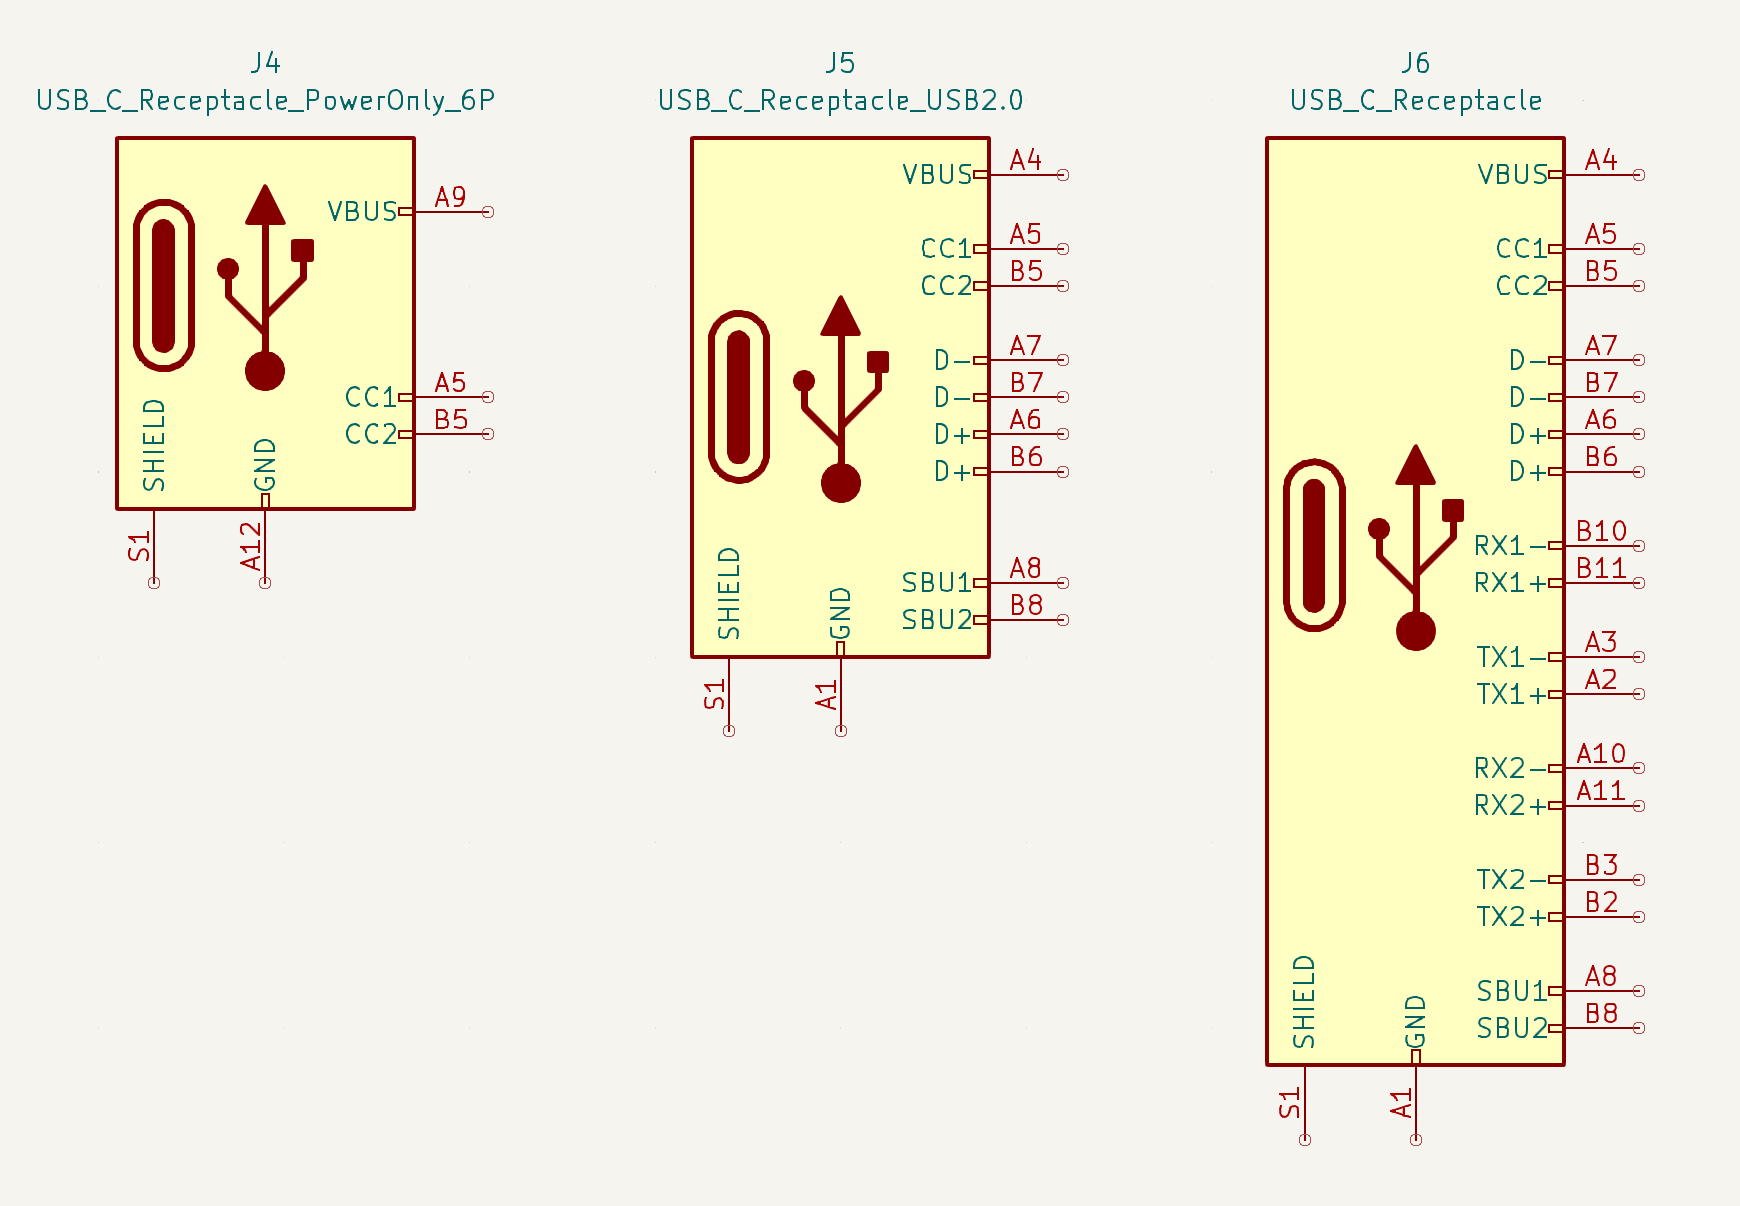
\includegraphics[width=1\linewidth]{images/3-USB-C.png}
	\caption{USB Type-C Selections}
	\label{fig:usbc-3-ports}
\end{figure}

Additionally, for reference, the pinout of a USB-C connector.\footnote{Figure 2, Microchip AN1953}


\begin{figure}[h]
	\centering
	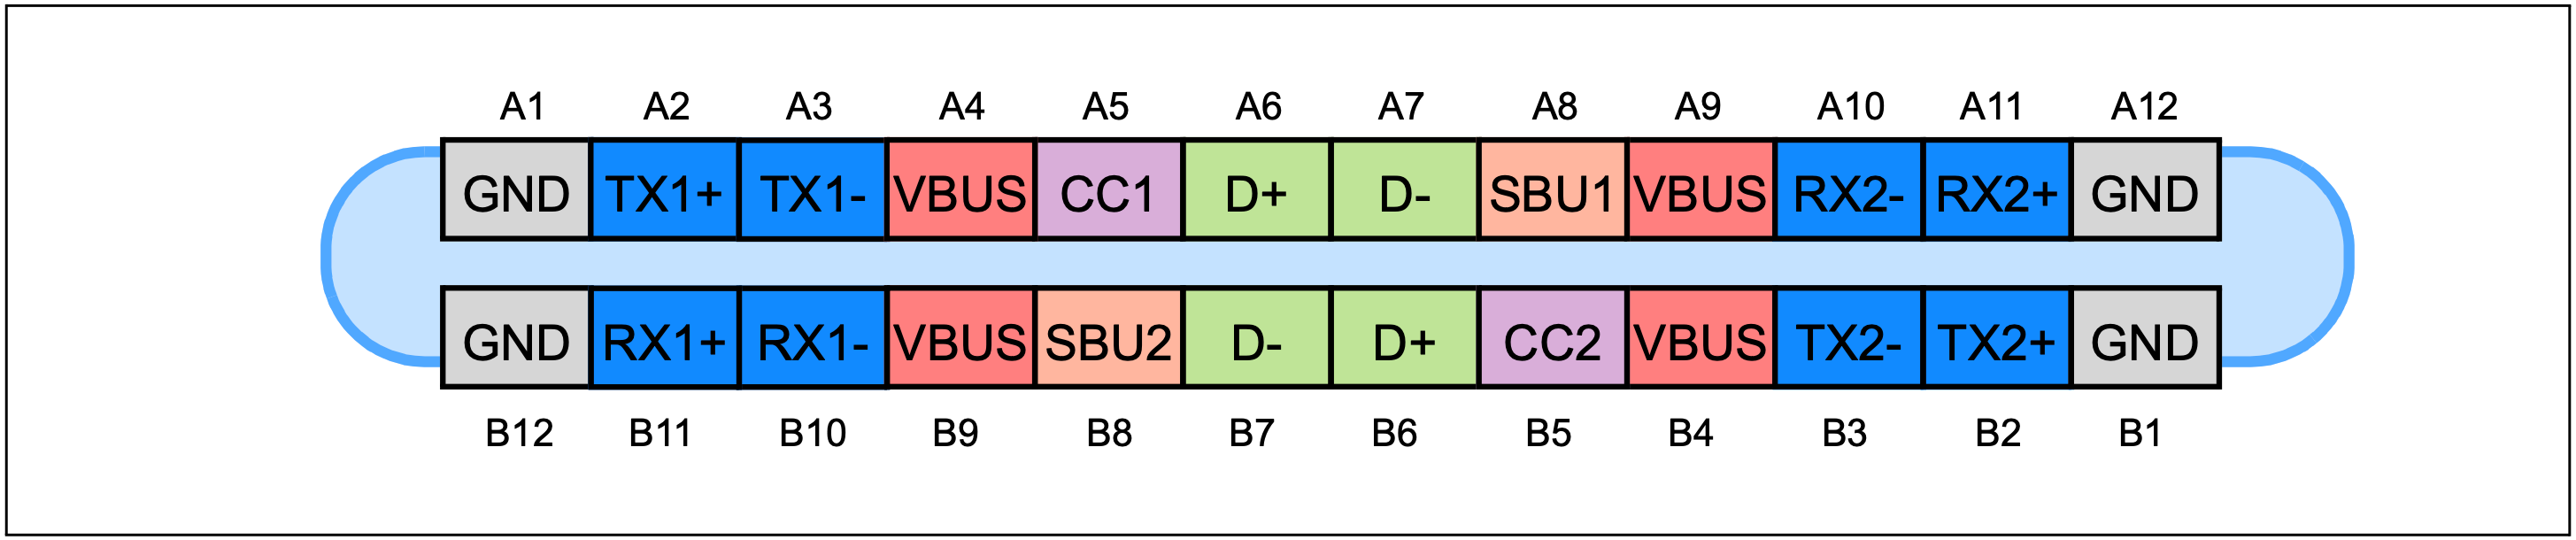
\includegraphics[width=1\linewidth]{images/microchip-pinout.png}
	\caption{USB-C Receptacle Pinout}
	\label{fig:usb-c-pinout-microchip}
\end{figure}

\newpage

\subsection{Power Only}

\begin{figure}[h]
	\centering
	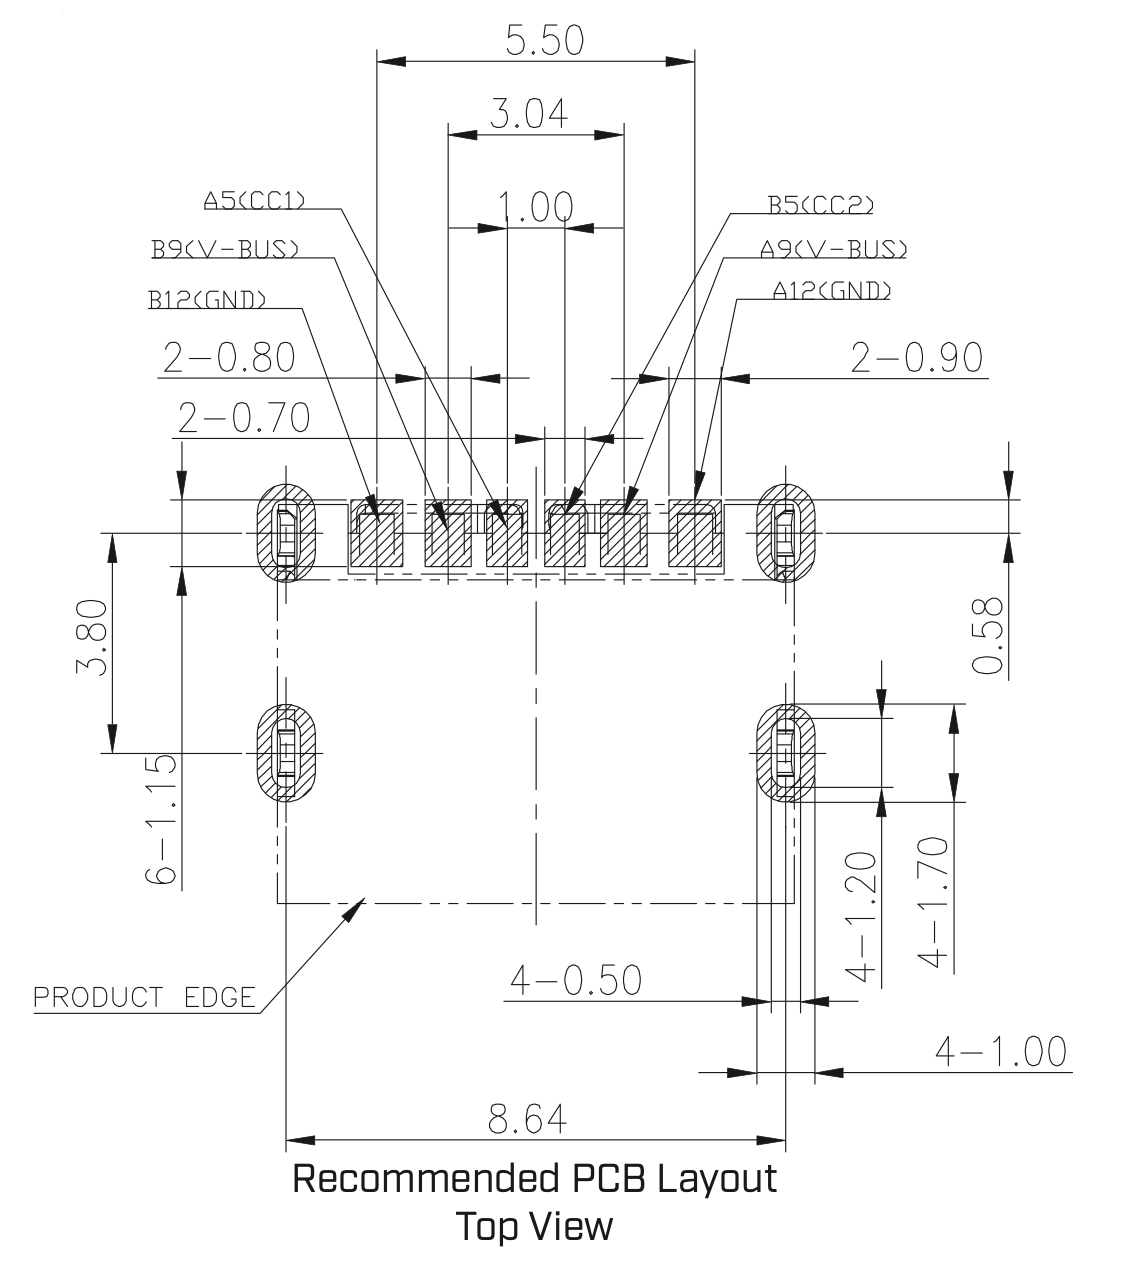
\includegraphics[width=.8\linewidth]{images/CUI-Devices-Power-Only.png}
	\caption{USB-C Power Only Pinout\protect\footnotemark}
	\label{fig:usb-c-pinout-power-only-CUI}
\end{figure}

\footnotetext{CUI Devices UJC-HP-3-SMT-TR}

\noindent
These connectors are very simple, having six pins each: VBUS, GND and CC on each side of the connector for a total of $3\cdot2 = 6$ pins. This does not support any data transfer and is much easier to route given the application that only requires power input. It has CC pins to allow for Power Delivery- though it's important to note not all connectors can support the full capability of Power Delivery- the UJC-HP-3-SMT-TR in the drawing shown only goes up to 20VDC and 3A on power pins together (1.5A individually). 


\newpage

\subsection{USB2 Type-C}

\begin{figure}[h]
	\centering
	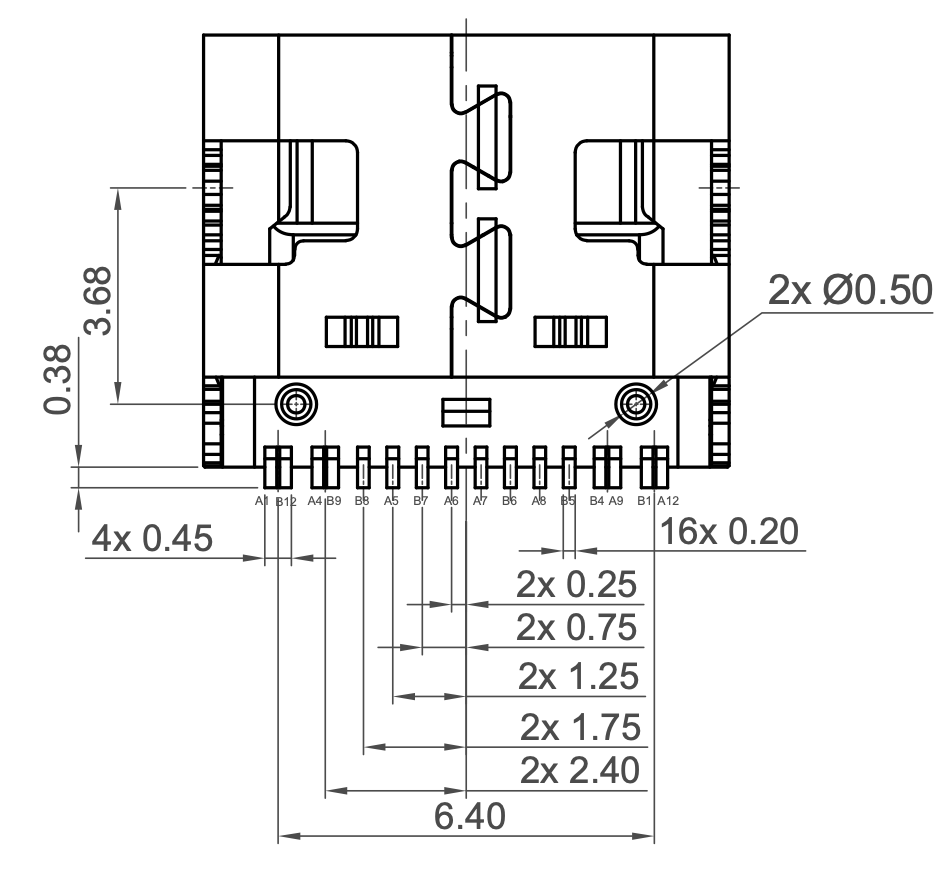
\includegraphics[width=.8\linewidth]{images/GCT-USB2-Type-C.png}
	\caption{USB2 Type-C\protect\footnotemark}
	\label{fig:usb-c-pinout-usb2-gct}
\end{figure}

\footnotetext{GCT Co USB4105}

\noindent
The USB2 connector has "12" pins as opposed to the standard expected 16 for USB2. This is due to some ingenious construction where they place the bottom and top GND / VBUS pins right next to each other, giving eight data pins and four "pairs" of power pins.\\\\
\noindent
It's quite simple to use for USB2 applications. You must connect VBUS and GND on either side of the connector, the CC circuitry, as well as the D+/- data pins.



\newpage

\subsection{USB3.2 Type-C}

\begin{figure}[h]
	\centering
	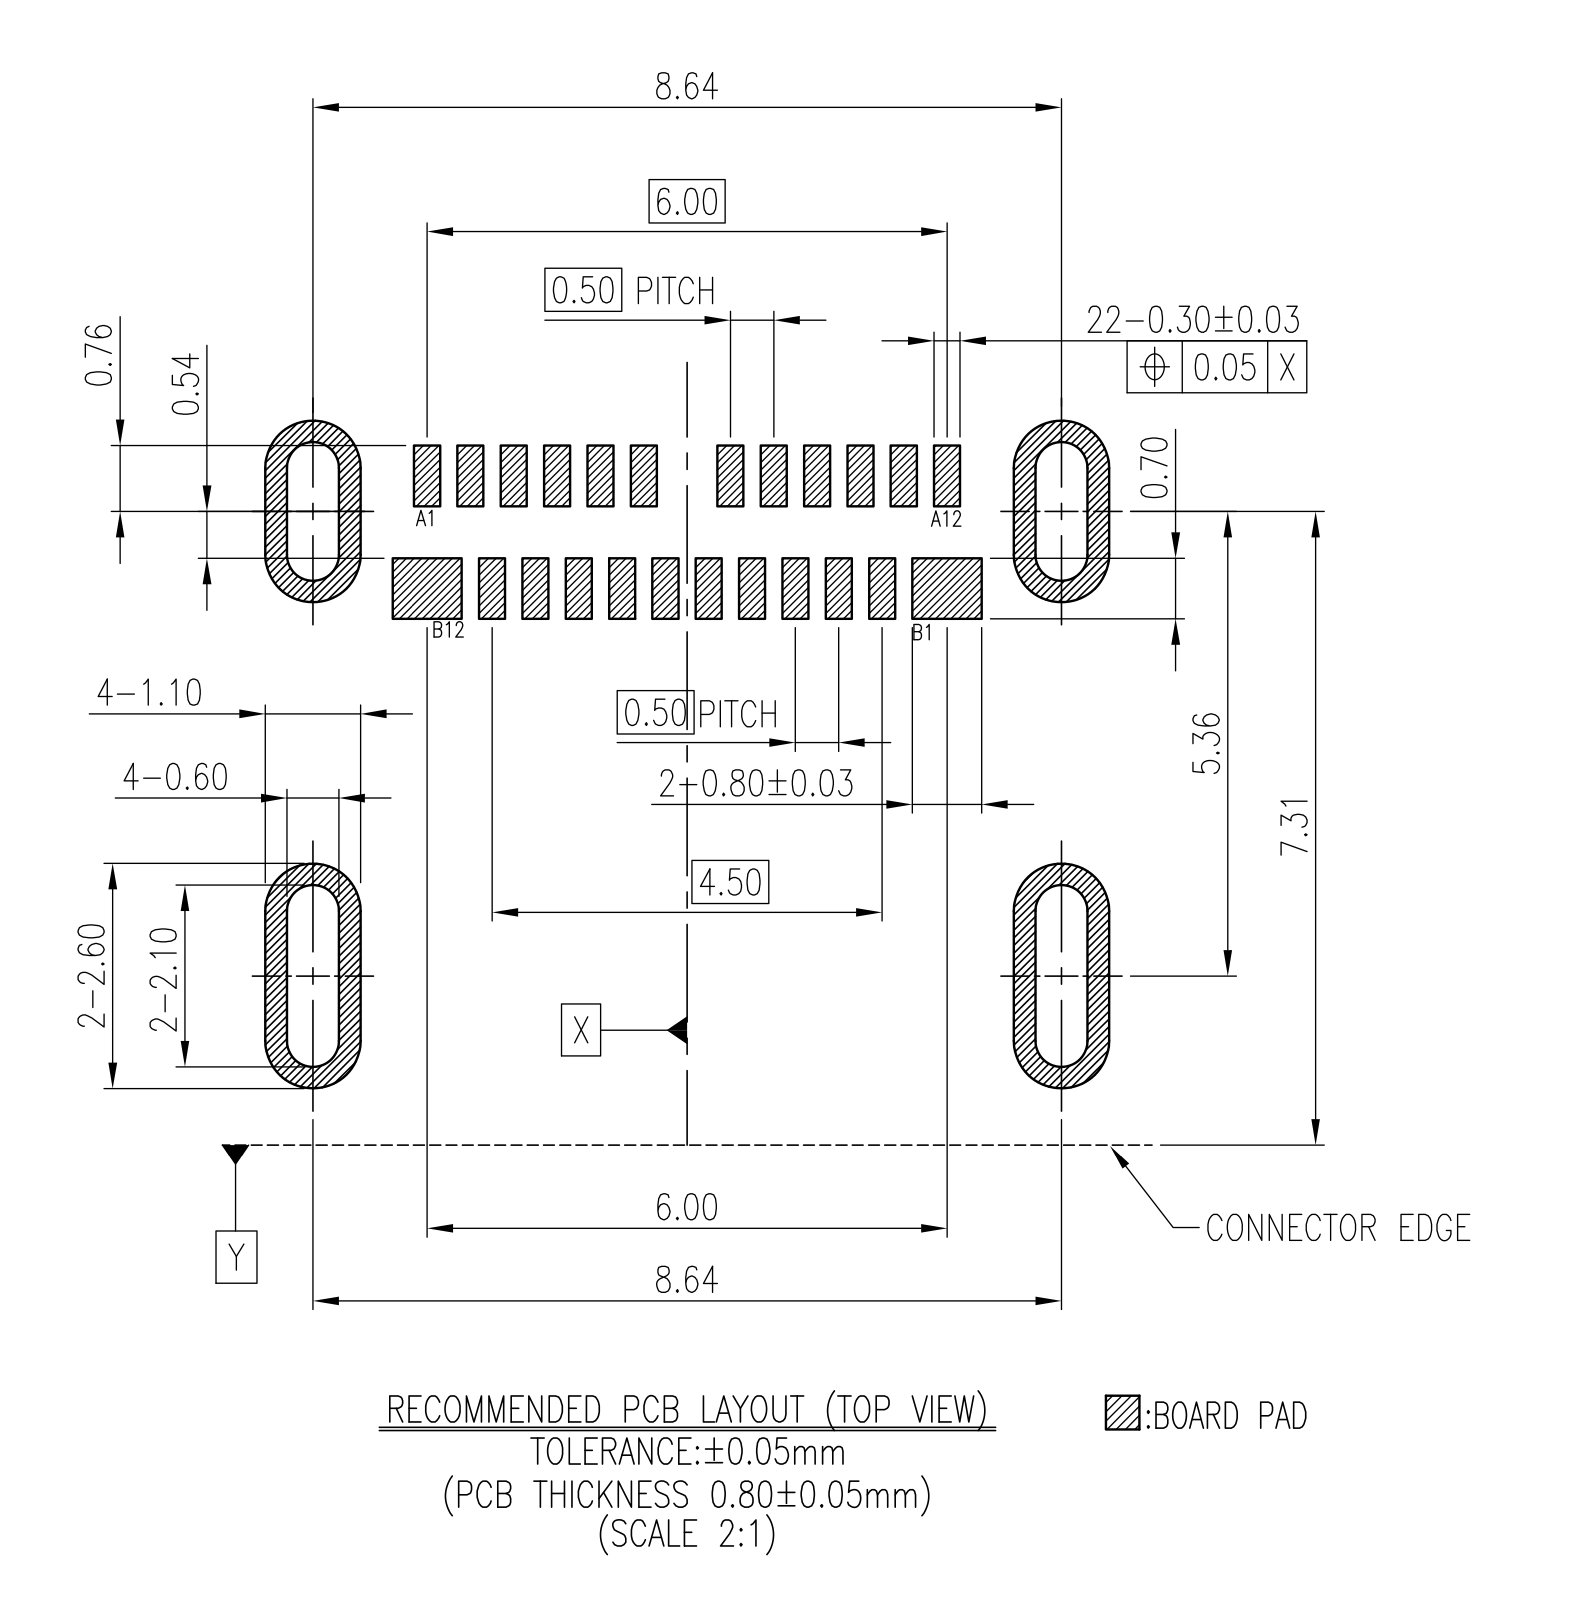
\includegraphics[width=.8\linewidth]{images/Amphenol-USB3.2-Type-C.png}
	\caption{USB3.2 Type-C\protect\footnotemark}
	\label{fig:usb-c-pinout-usb3.2-amphenol}
\end{figure}

\footnotetext{Amphenol Corp GSB3C31X3DSYHR}

\noindent
In order to implement the full USB3 (or USB4!) functionality, an additional two pairs of data pins are needed: TX+/- and RX+/-. This is an extra eight pins (four on each side) for a total of 24 pins. Unless you need USB3, it's generally a bad idea to use these connectors: they're more expensive, harder to route, and generally no benefit over a USB2 connector if your circuit is USB2. 


\newpage
\section{Power Delivery}

As mentioned earlier in \ref{sec:AnalogPower}, you can get 5V at higher current levels than USB2-capability with the addition of 5.1K$\Omega$ ± 10\% pulldown resistors on CC1 and CC2. However, it is impossible to negotiate higher voltage levels with resistors, and you'll need a dedicated USB Type-C port controller. Most of these aren't incredibly difficult to implement, but vary in capability and usage. \\\\
\noindent
There are a few ways various chips expect you to configure voltage and current setting. Typically, it's one of the three:
\begin{itemize}
	\item Flashing setting to controller's onboard non-volatile storage
	\item Controlled through MCU (eg, STUSB4500)
	\item Controlled through resistor values (eg, CYPD3177)\\
\end{itemize}

\noindent
While not all PD controllers support all these function, the more powerful ones do:
\begin{itemize}
	\item Voltage settings (5V, 9V, 12V, 15V, 19V, 20V)
	\item Fine Current Adjustment 
	\item Coarse Current Adjustment (up to 5A)
	\item Some ability to control via $I^2 C$\\
\end{itemize}

\noindent
A tested board based on the CYPD3177-24LQXQ, built for \href{https://github.com/hackclub/blot/tree/main}{Blot}, is open source and available \href{https://github.com/Hugoyhu/CYPD3177-Breakout}{here}. An export of the schematic capture is available on the next page.\\

\noindent
It's important to note that PD applications should be considered carefully. Power Delivery can provide above 5V of power, but not all applications can withstand high voltages and currents. One example would be having the output of a PD board be a standard USB-A connector. While this may seem like an OK idea in practice, it should be important to remember that the expected power from a USB-A port is 5V, and mistakingly configuring your PD output as 9V or above will likely destroy whatever's connected to the port.
 
\newpage
\begin{figure}[h]
	\centering
	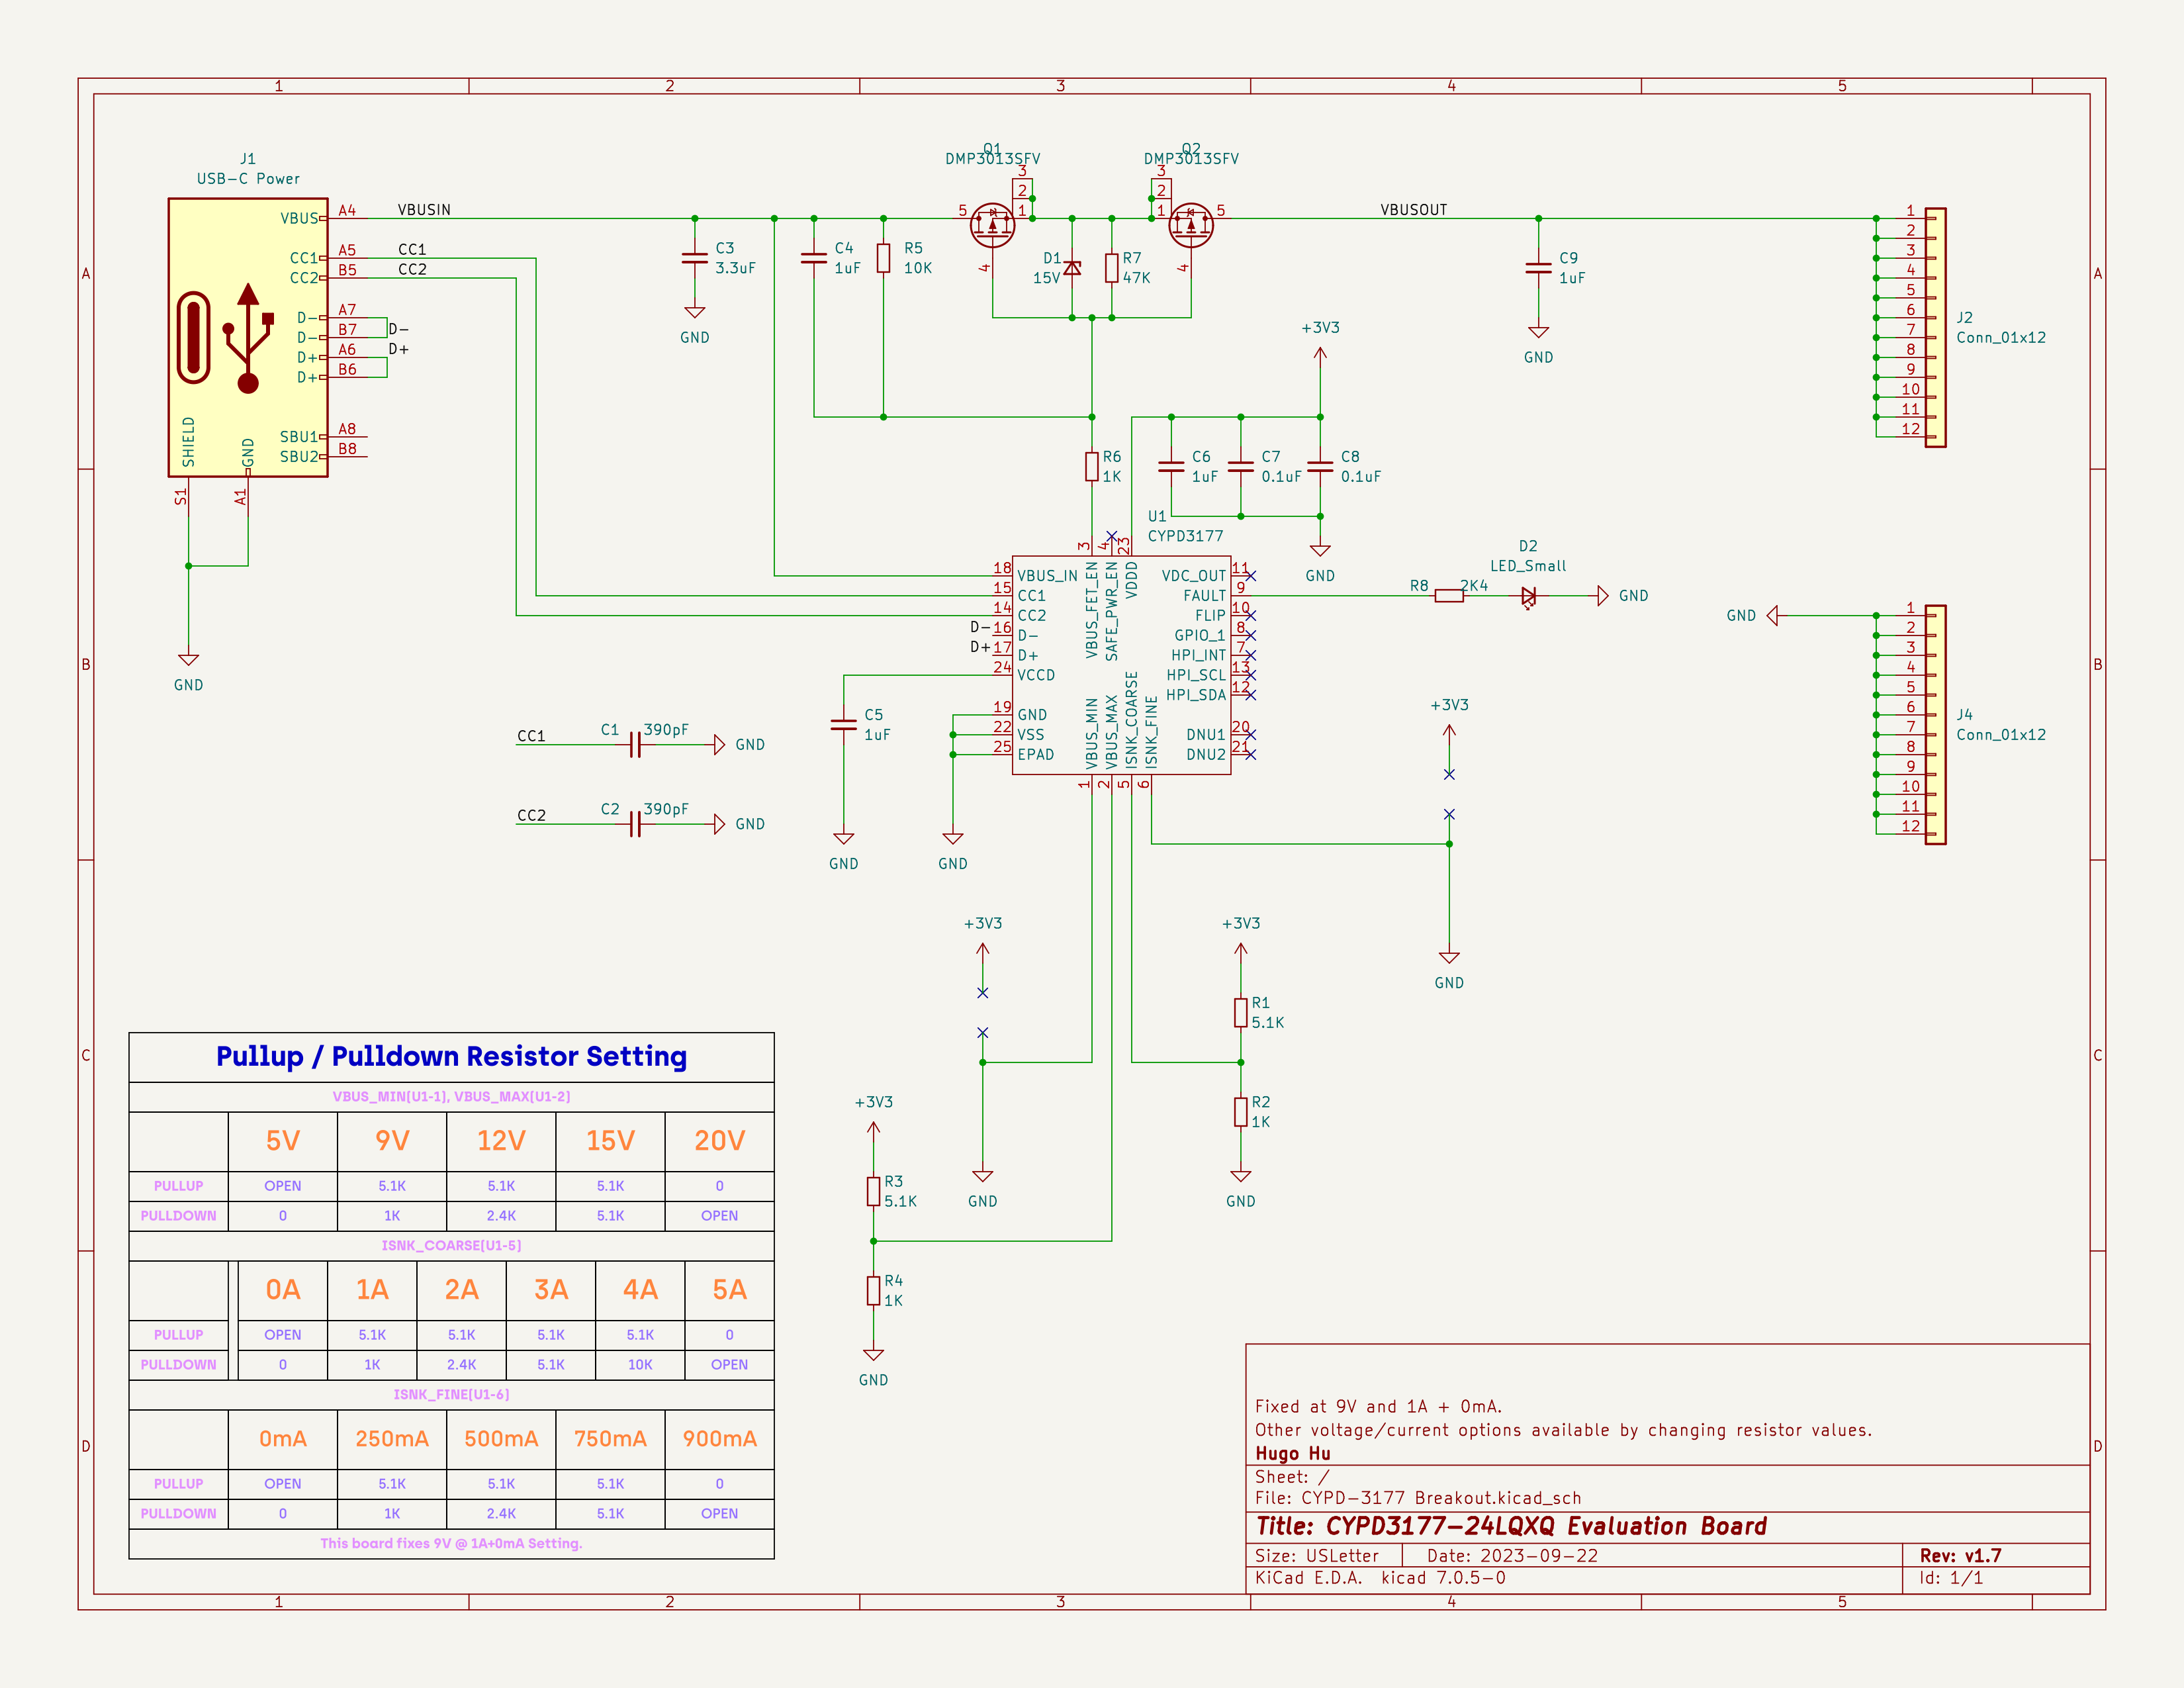
\includegraphics[width=\linewidth]{images/CYPD3177_sch.png}
	\caption{CYPD3177 Schematic Capture\protect\footnotemark}
	\label{fig:cypd3177_sch}
\end{figure}

\footnotetext{\href{https://github.com/Hugoyhu/CYPD3177-Breakout/blob/main/CYPD3177\%20Breakout\%20Schematic.png}{Image Source}}

\newpage

\section{Downstream USB-C Ports}

We can now do a lot with a USB-C input, but what about converting a downstream facing USB-A port to USB-C? For example, if we had a USB hub with USB2.0 Type-A outputs, and wanted to make them USB2.0 Type-C. It's not necessarily as easy as simply adding the port, but close enough. We just need two CC resistors, one on each pin. 

\begin{figure}[h]
	\centering
	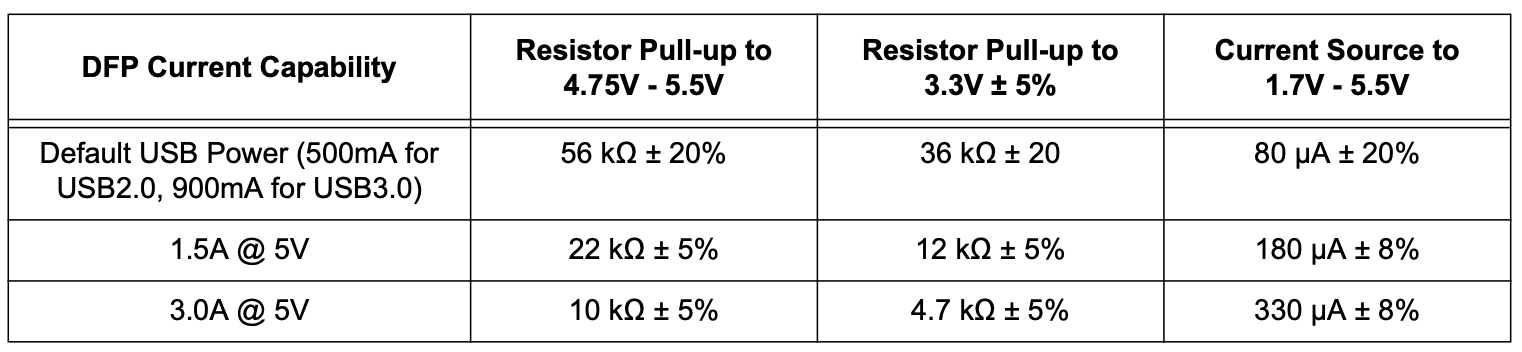
\includegraphics[width=\linewidth]{images/microchip-dfp-table.png}
	\caption{DFP Resistor Chart\protect\footnotemark}
	\label{fig:microchip_dfp}
\end{figure}

\footnotetext{Microchip AN1953 DFP Resistor Chart}

\noindent
To convert a traditionally USB2.0 design, it's most likely that the design only supports 500mA (Default Power), so in most cases, two 56K$\Omega$  ± 20\% pull-up resistors should be sufficient. If your design receives external power, then it's a good idea to consider increasing maximum current to 1.5A or 3.0A with the resistor pull-up values specified. \\


\noindent
For example, this USB2 hub design takes existing USB-A outputs and converts them to USB-C out. Keep in mind, changing the connector doesn't actually give you any increase in speed- a USB2 design will continue to operate at USB2 speeds even with USB-C. 

\newpage
\begin{figure}[h]
	\centering
	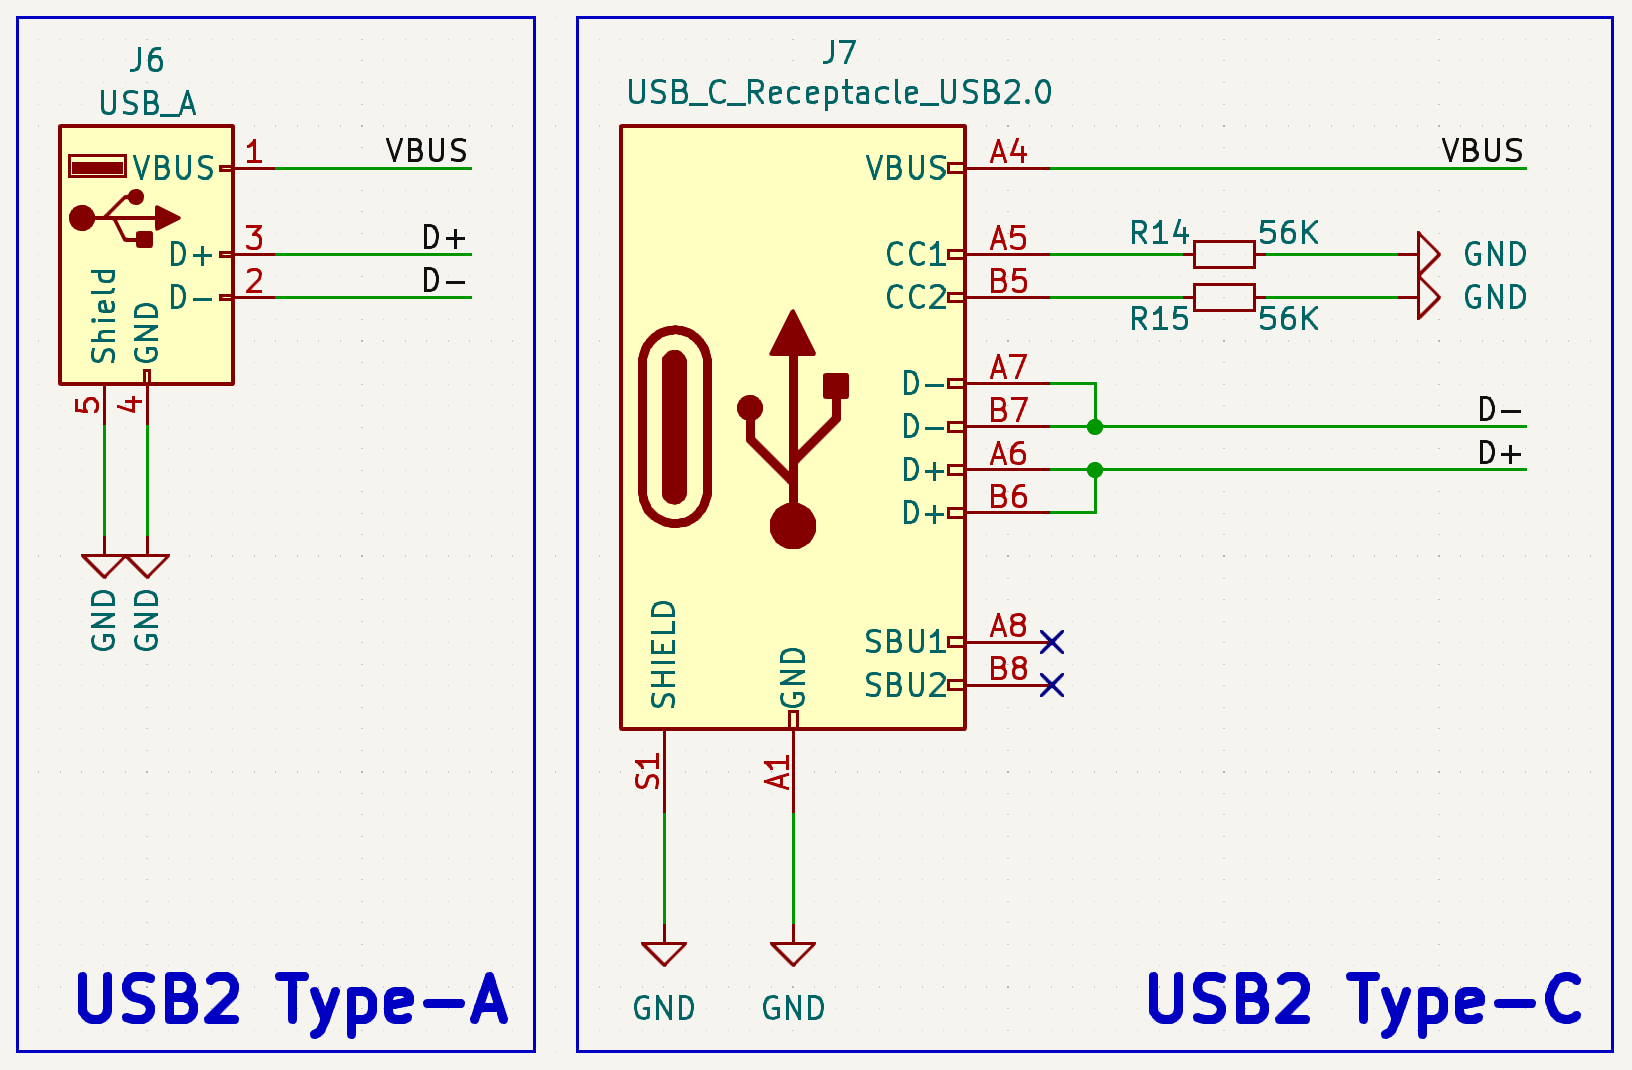
\includegraphics[width=\linewidth]{images/USBAtoUSBC.png}
	\caption{USB Type-A vs USB Type-C 500mA Power}
	\label{fig:usbconversion}
\end{figure}

\begin{figure}[h]
	\centering
	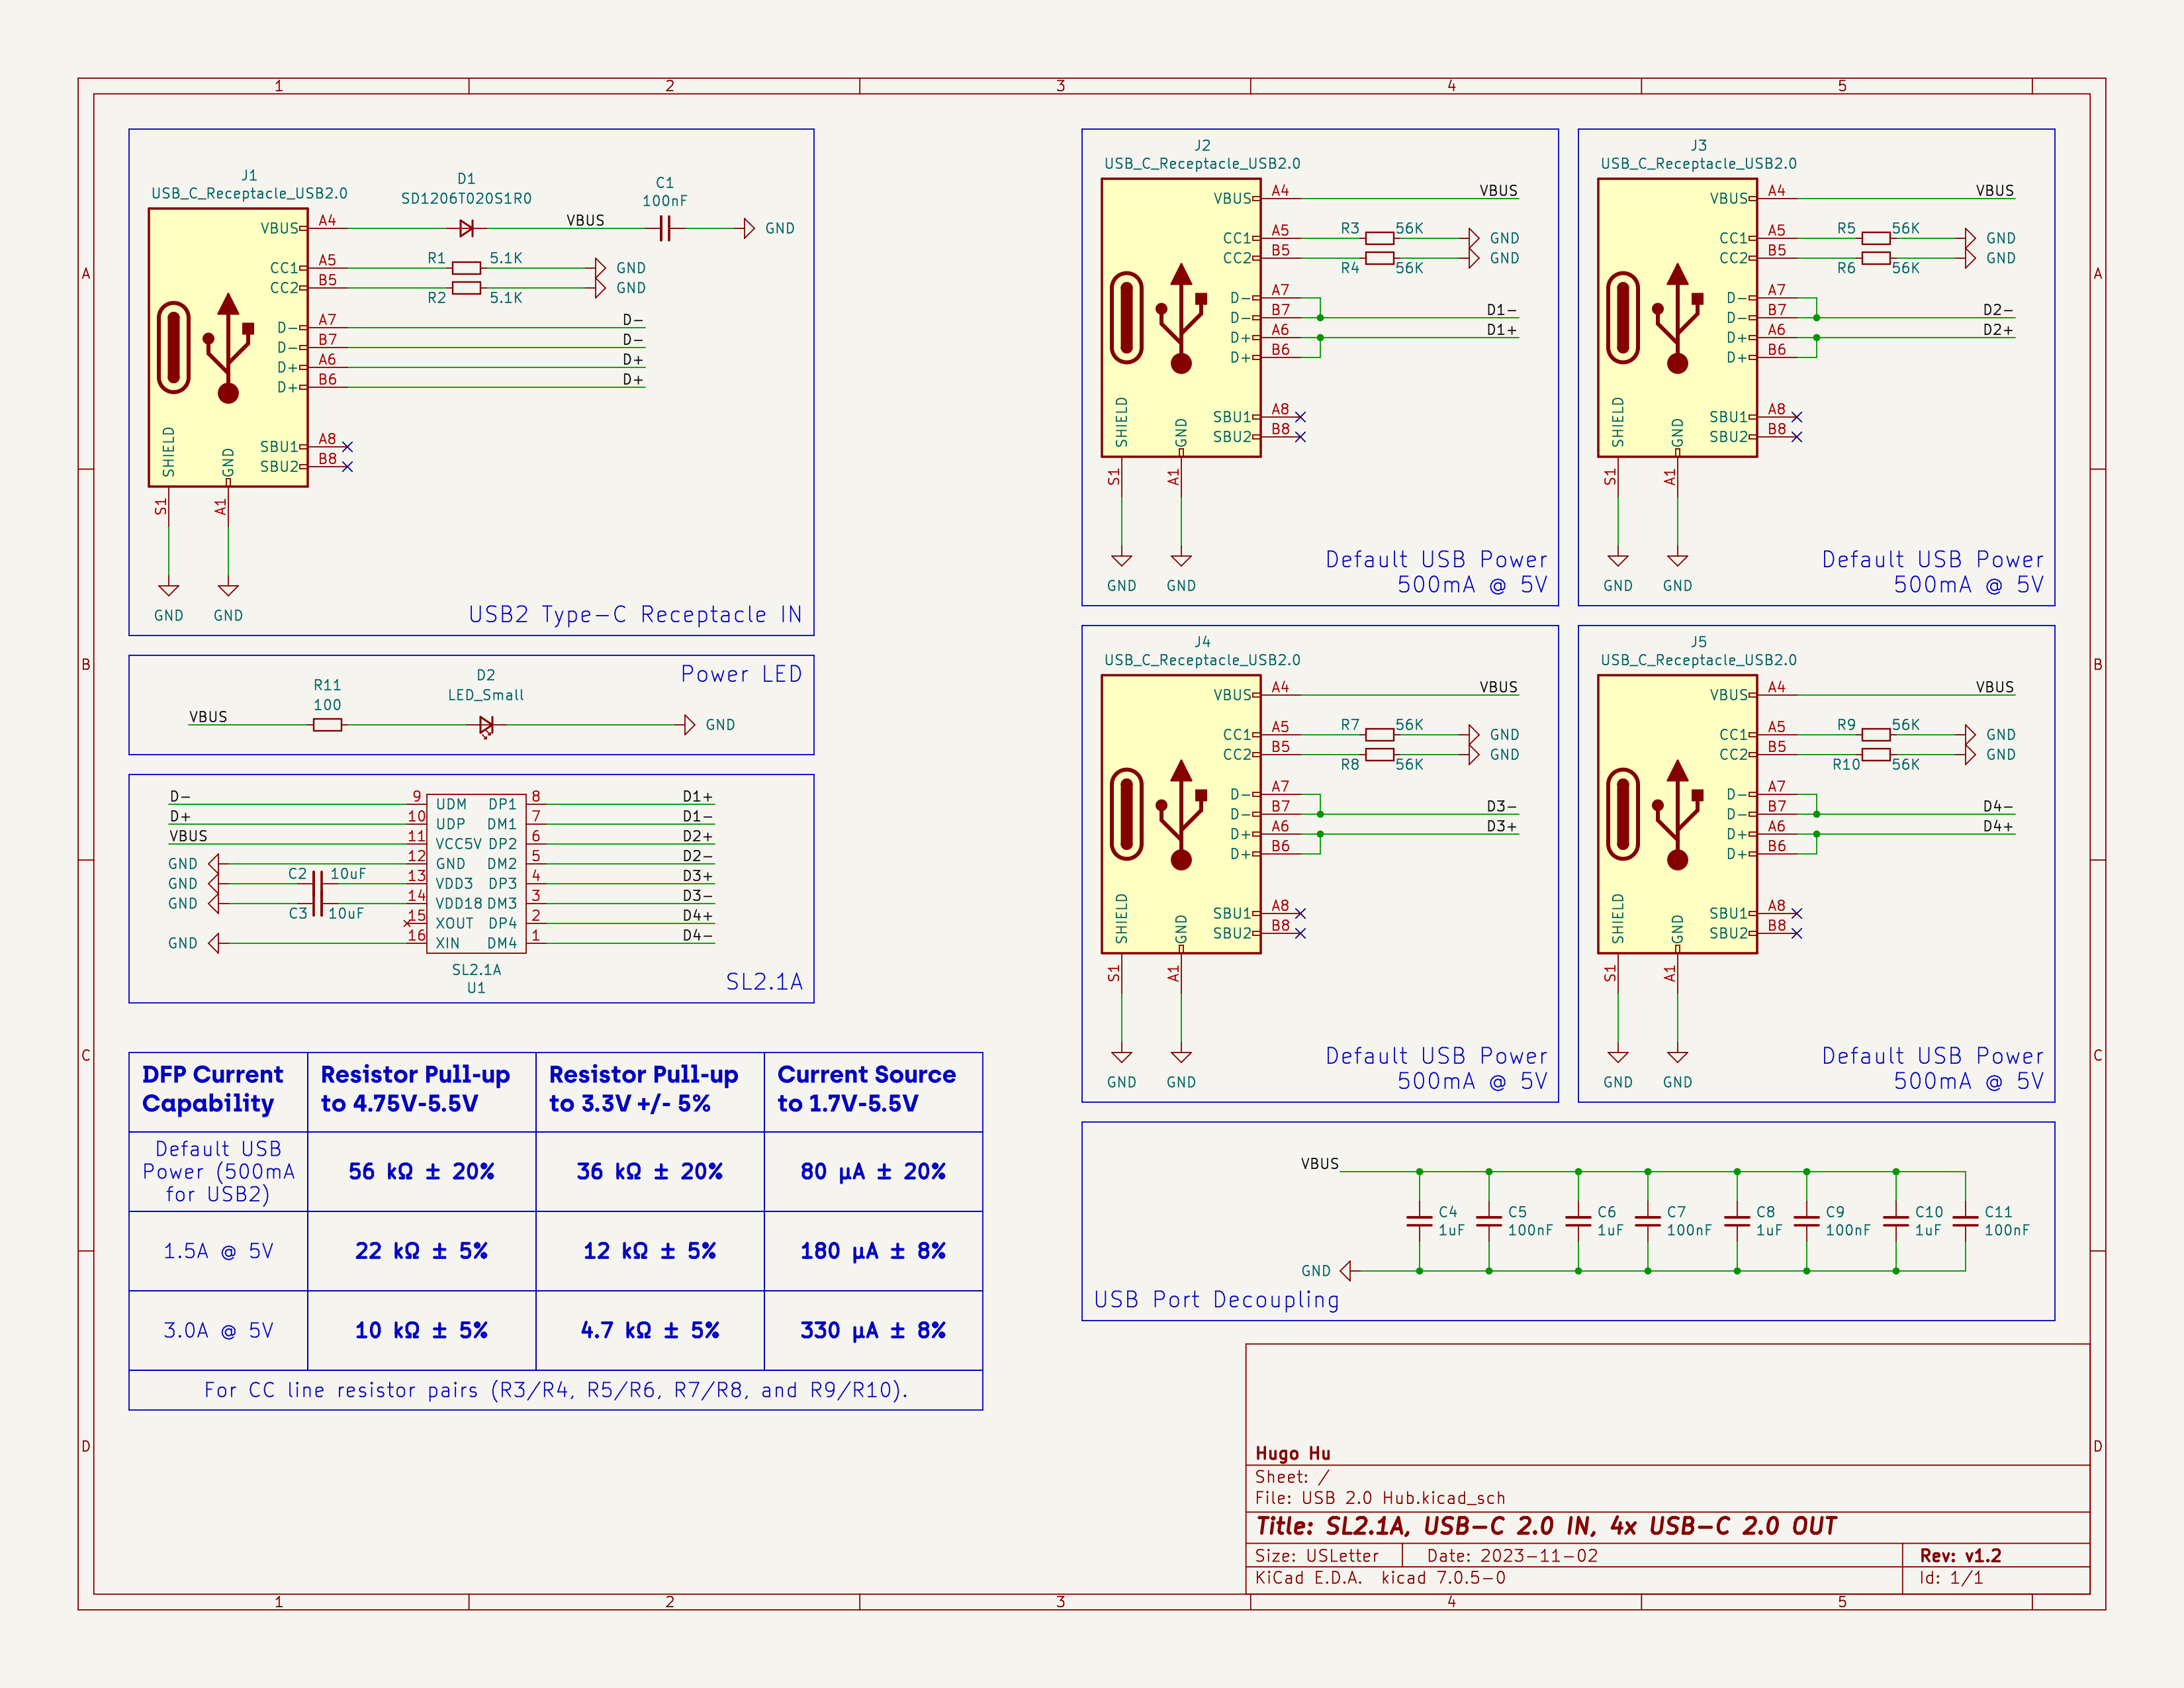
\includegraphics[width=\linewidth]{images/SL2.1A.png}
	\caption{SL2.1A based USB2 Type-C hub\protect\footnotemark}
	\label{fig:sl21a}
\end{figure}
\footnotetext{Can be found here: https://github.com/Hugoyhu/SL2.1A-Type-C-Hub}

\newpage
\section{Conclusion}
\noindent
This document is hardly a comprehensive source for USB-C. This is more-so an introduction to new features offered by the USB-C standard. The information here is mostly accurate (for most applications) for a USB2 application, but lacks much critical information for a USB3+ based design. It's also important to note that not all information here is complete, and may at times be a simplification. 
For more information about the USB-C spec and implementation, you should take a look at the further reading below. 

\newpage

\section{Further Reading}

\href{https://ww1.microchip.com/downloads/en/appnotes/00001953a.pdf}{Microchip Application Note 1953: Introduction to USB Type-C}\\\\
\href{https://www.ti.com/lit/wp/slyy109b/slyy109b.pdf?ts=1696814775662}{Texas Instruments: A Primer on USB Type-C and USB Power Delivery Applications and Requirements}\\\\
\href{https://www.st.com/resource/en/technical_article/dm00496853-overview-of-usb-type-c-and-power-delivery-technologies-stmicroelectronics.pdf}{ST Microelectronics TA0357: Overview of USB Type-C and Power Delivery Technologies}\\\\













\end{document}